%!TEX root=../document.tex

\section{Ergebnisse}
\label{sec:Ergebnisse}
\subsection{C++ Kompilieren und Ausführen}
Der erste Schritt war es C++ kompilieren zu können. Da ich auf Linux arbeite, kann ein \verb|.cpp| File folgendermaßen kompiliert und ausgeführt werden:

\begin{lstlisting}[language=bash]
g++  ${file} -std=c++1z -o ${fileBasenameNoExtension}  && ./${fileBasenameNoExtension}
\end{lstlisting}

\subsection{Topologie und Parameter anpassen}
Da die Aufgabe \textbf{3} Inputs und \textbf{3} Outputs erwartet, muss die Topologie angepasst werden. Es wurde sich für einen Hidden Layer mit \textbf{5} Nodes entschieden, dadurch ergibt sich folgende Liste an Integer als Parameter:

\begin{lstlisting}[language=c]
	topologie{ 3,5,3 }
\end{lstlisting}

Weiters wurde statt der \verb|ReLU| Funktion eine Sigmoid-Funktion (\verb|eins_durch_ehoch|) verwendet kombiniert mit einer \verb|learnRate| von \textbf{0.9} statt \textbf{0.09} 
\subsection{NN trainieren}
Um das Netz zu trainieren wurden das Trainingset angepasst:

\begin{lstlisting}[language=c]
	// Beispiel fuer 001 -> 011
	p->input[0] = 0.0;
	p->input[1] = 0.0;
	p->input[2] = 1.0;
	p->trueVal[0] = 0.0;
	p->trueVal[1] = 1.0;
	p->trueVal[2] = 1.0;
	p->calc(learn{ true });
\end{lstlisting}
\clearpage
\subsection{Ausgabe}
Natürlich musste auch die Angabe angepasst werden, da nun statt \textbf{2} Inputs und \textbf{1} Output jeweils \textbf{3} Inputs und \textbf{3} Outputs vorhanden sind. Beim Ausführen ergibt sich folgende Ausgabe:

\begin{minipage}{\linewidth}
	\centering
	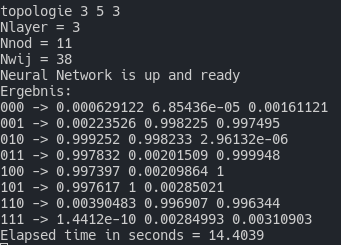
\includegraphics[width=0.8\linewidth]{images/sc}
\end{minipage}
